\section{eo\-Boolean\-Generator Class Reference}
\label{classeo_boolean_generator}\index{eoBooleanGenerator@{eoBooleanGenerator}}
The class eo\-Boolean\-Generator can be used in the STL generate function to easily generate random booleans with a specified bias.  


{\tt \#include $<$eo\-Rnd\-Generators.h$>$}

Inheritance diagram for eo\-Boolean\-Generator::\begin{figure}[H]
\begin{center}
\leavevmode
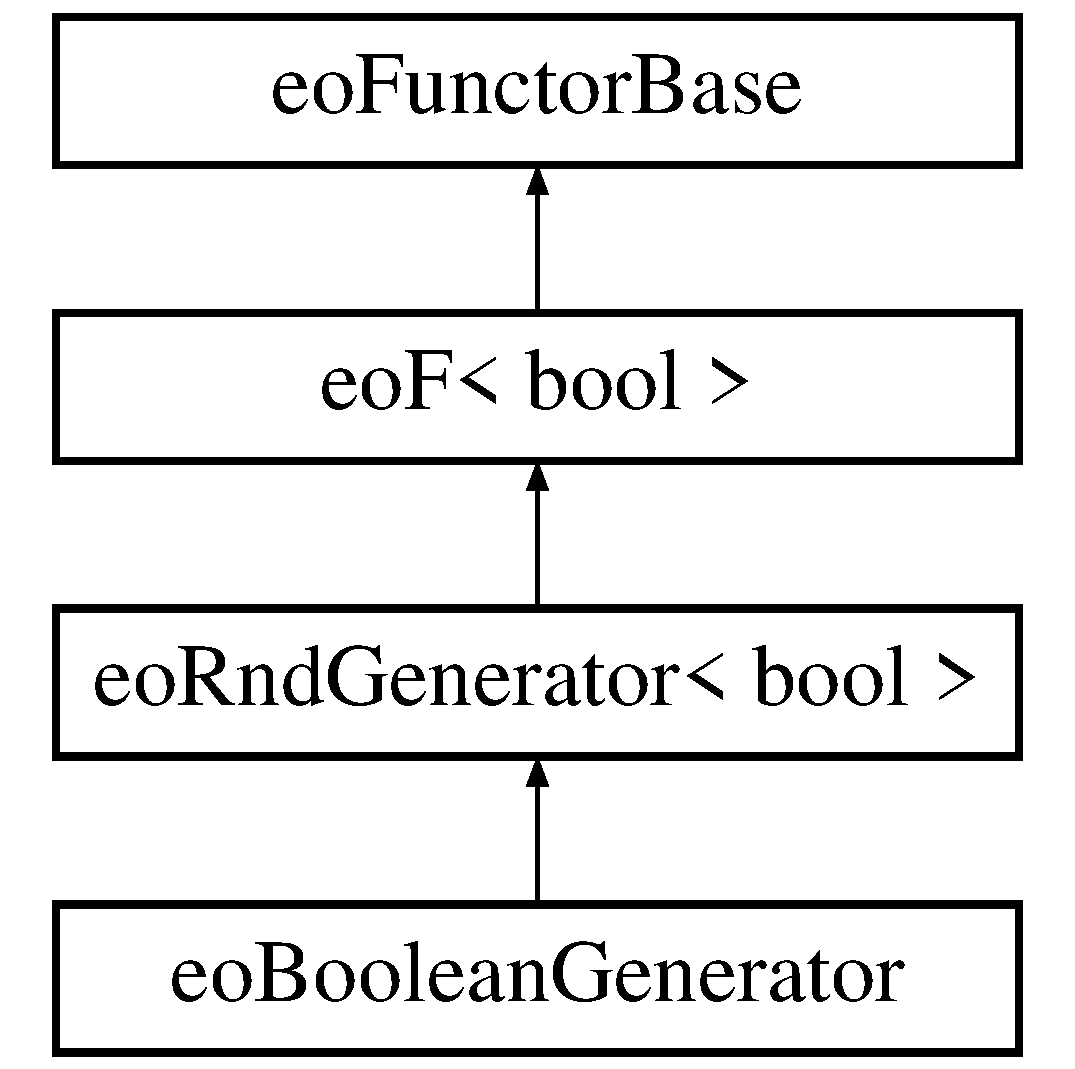
\includegraphics[height=4cm]{classeo_boolean_generator}
\end{center}
\end{figure}
\subsection*{Public Member Functions}
\begin{CompactItemize}
\item 
{\bf eo\-Boolean\-Generator} (float \_\-bias=0.5, {\bf eo\-Rng} \&\_\-rng=rng)\label{classeo_boolean_generator_a0}

\item 
bool {\bf operator()} (void)\label{classeo_boolean_generator_a1}

\begin{CompactList}\small\item\em The pure virtual function that needs to be implemented by the subclass. \item\end{CompactList}\end{CompactItemize}
\subsection*{Private Attributes}
\begin{CompactItemize}
\item 
float {\bf bias}\label{classeo_boolean_generator_r0}

\item 
{\bf eo\-Rng} \& {\bf gen}\label{classeo_boolean_generator_r1}

\end{CompactItemize}


\subsection{Detailed Description}
The class eo\-Boolean\-Generator can be used in the STL generate function to easily generate random booleans with a specified bias. 



Definition at line 104 of file eo\-Rnd\-Generators.h.

The documentation for this class was generated from the following file:\begin{CompactItemize}
\item 
eo\-Rnd\-Generators.h\end{CompactItemize}
